\documentclass[12pt]{article}

\usepackage{tcolorbox}
\usepackage[english]{babel}
\usepackage[utf8x]{inputenc}
\usepackage[T1]{fontenc}
\usepackage{url}
\usepackage{listings}
\usepackage{braket}
\usepackage{graphicx} % Required for inserting images
\usepackage{color}
\usepackage{mdframed}
\usepackage{amsmath}
\usepackage{amsfonts}
\usepackage{wrapfig}
% \usepackage{fullpage}
\usepackage{hyperref}

\begin{document}

\begin{titlepage}
    \begin{center}
        \Huge
        \vspace*{\fill}
        Analyzing Decision-Making in the 2D Random Dot Motion Discrimination Task Using the Drift Diffusion Model

        \vspace{3cm}
        \Large
        Ryan Carroll \& Mohammed Abbasi

        \vspace{3cm}
        April 16, 2025

        \vspace{3cm}
        Rensselaer Polytechnic Institute

        \vspace*{\fill}
    \end{center}
\end{titlepage}

\section{Introduction}

This project addresses data gathered from a 2D random dot motion discrimination task. In this task, participants are presented with a two-axis grid resembling an `X.' Each axis has a red platform at one end and a blue one at the other. Balls move along each axis, and participants are asked to determine which colored platform (red or blue) has more dots moving towards it (see Figure \ref{fig:task}). There were multiple variables recorded in this study. One such variable is focus on one or both axes; in some scenarios, participants only have to focus one one axis, which has white balls (the other has black balls). In other scenarios, both axes have white balls, meaning participants must focus on both axes \cite{krzeminski_zhang_2020}. Here, however, we focus only on how the angle of the axes affects participants' during the experiment. Specifically, we analyze response times (RT) and accuracy data from a single participant performing this task with axes at two different angles (20° and 45°) to determine differences in cognitive processing.
\begin{figure}[ht]
    \centering
    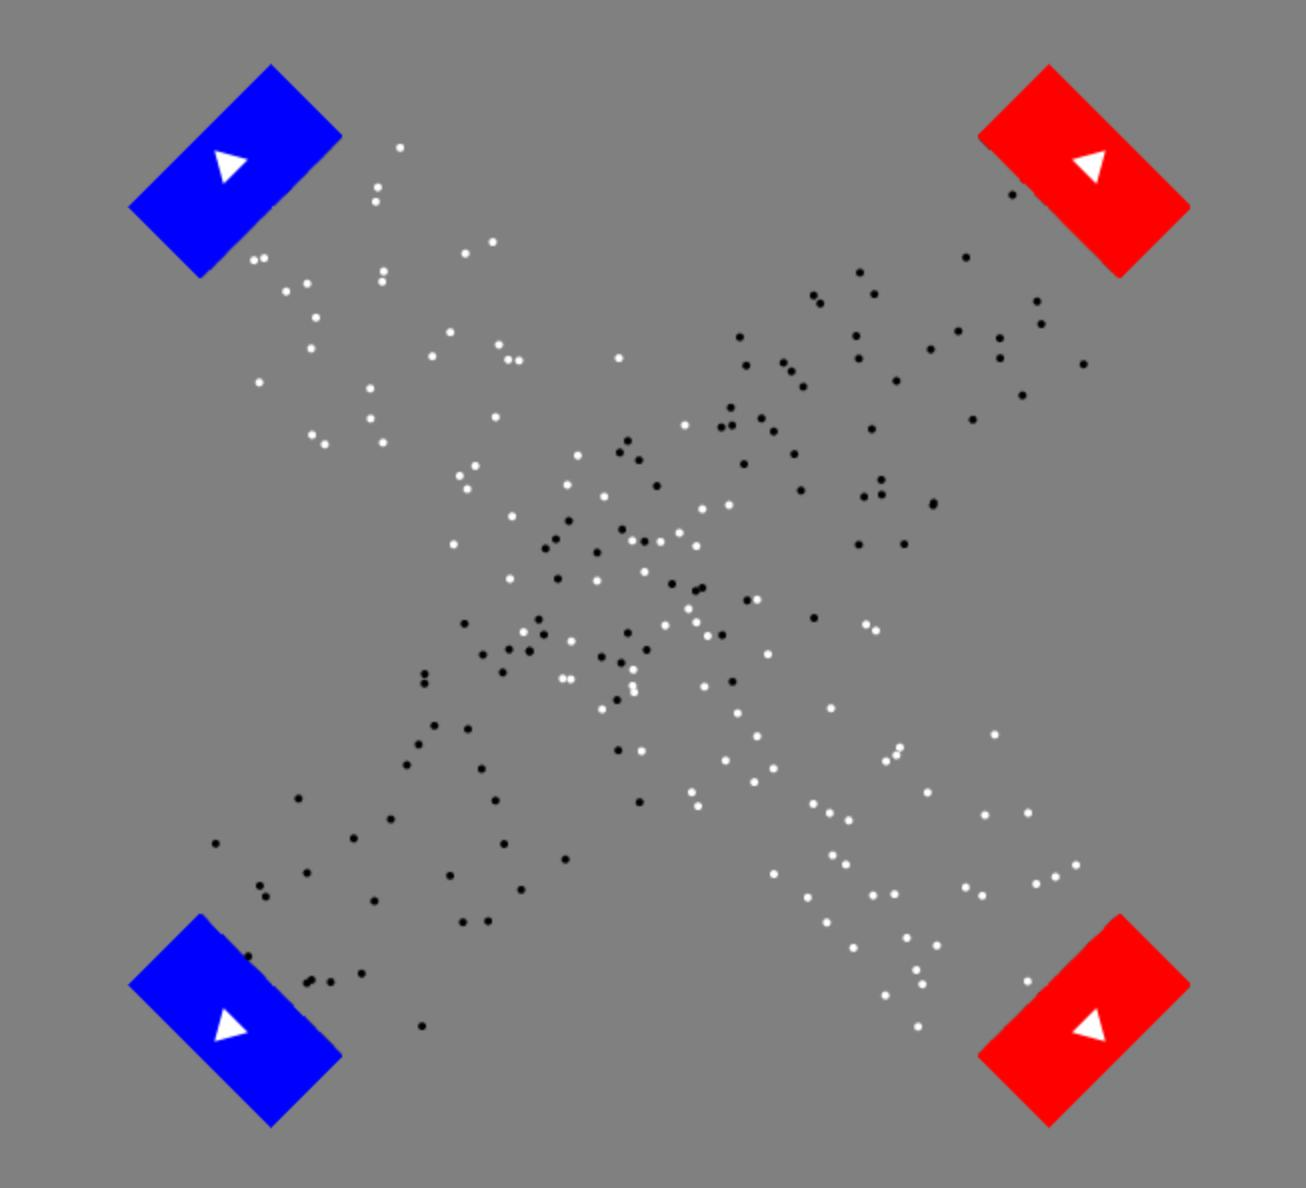
\includegraphics[width=0.5\textwidth]{2drdk_part1.2400x2400.jpeg}
    \caption{The 2D random dot motion discrimination task. The participant must determine which colored platform has more dots moving towards it.}
    \label{fig:task}
\end{figure}

\section{Methods}
\subsection{Model}
We utilized a Drift Diffusion Model (DDM), which is widely used in decision-making research. The model assumes decision-making as evidence accumulation over time until a boundary, the decision threshold, is reached. This model follows a Wiener process, which is a stochastic process that models continuous-time motion with random and independent motion. The parameters of this model are:
\begin{itemize}
    \item Drift rate ($v$): the rate at which evidence is accumulated.
    \item Boundary separation ($a$): the amount of evidence required to make a decision.
    \item Non-decision time ($\tau$): the time taken by processes before decision-making begins.
    \item Starting bias ($\beta$): the initial position of evidence accumulation, which represents bias toward a response.
\end{itemize}
We set the Priors for these parameters as follows:
\begin{itemize}
    \item $v \sim \text{Gamma}(3, 1)$
    \item $a \sim \text{Gamma}(3, 1)$
    \item $\tau \sim \text{Gamma}(2, 1)$
    \item $\beta \sim \text{Beta}(2, 2)$
\end{itemize}
These distributions are visually represented in Figure \ref{fig:priors}. All of these priors are weakly informative, meaning they do not strongly influence the posterior distributions. This is done because we have limited knowledge of the domain and want to allow the data to inform the model as much as possible.
\begin{figure}[ht]
    \centering
    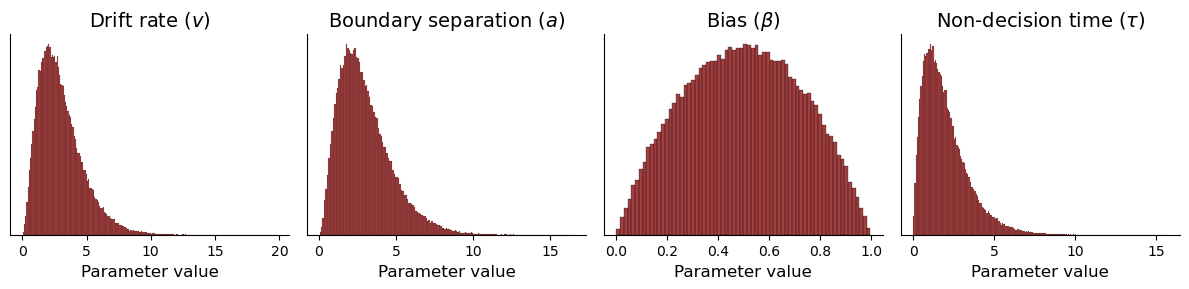
\includegraphics[scale=.45]{priors.png}
    \caption{A visual representation of prior distributions. The priors are weakly informative, allowing the data to inform the model.}
    \label{fig:priors}
\end{figure}
\subsection{Data and Software}
We analyze RT and correctness data from one participant's 20° and 45° datasets \cite{Krzeminski2021}, each containing just under 600 trials. Python is used to clean and filter the dataset. Stan (via PyStan) is used to perform Bayesian parameter estimation leveraging Markov Chain Monte Carlo (MCMC) sampling. Other libraries include:
\begin{itemize}
    \item NumPy for numerical operations.
    \item Pandas for data manipulation via DataFrames.
    \item Matplotlib, Seaborn, and Arviz for data visualization.
\end{itemize}

\subsection{Model Diagnostics and Validation}
Model convergence is verified using R-hat statistics and visual posterior density plots to ensure chains are well-mixed. Predictive performance is validated by generating synthetic DDM data using the mean of the estimated parameters as arguments for the Python function we created in class. This synthetic data is visually compared to the original data to ensure a similar distribution. The model is fit using 4 chains with 2000 iterations and 1000 warmup iterations each.

\section{Results}
\subsection{Diagnostics}
The MCMC diagnostics indicated convergence (R-hat values for all parameters $\approx 1.0$). Posterior distributions were stable across chains. Standard deviations were all $< 0.1$, indicating low variability in parameter estimates. 

\subsection{Interpretation}
The 20° task yielded a mean drift rate ($v$) of approximately 0.71, boundary separation ($a$) of approximately 1.95, non-decision time ($\tau$) of approximately 0.50 seconds, and starting bias ($\beta$) of approximately 0.56. The 45° task yielded a mean drift rate ($v$) of approximately 0.87, boundary separation ($a$) of approximately 2.05, non-decision time ($\tau$) of approximately 0.32 seconds, and starting bias ($\beta$) of approximately 0.56. To summarize: when given a 45° angle, the drift rate is higher, indicating faster evidence accumulation. The boundary separation is also higher, indicating that the participant requires more evidence to reach a decision. The non-decision time is lower for the 45° angle, indicating that the participant is able to make decisions faster when given a 45° angle. The starting bias is similar across both angles, indicating that the participant has a slight bias toward one option over the other in either situation.

\subsection{Validation}
For both datasets, we generated synthetic RT data using the mean of the posterior distributions for each parameter (Figures \ref{fig:20deg} and \ref{fig:45deg}). The synthetic data was generated using the same number of trials as the original datasets (approximately 600). We then plotted the empirical and synthetic RT distributions for both conditions (20° and 45°) to visually assess model fit. The synthetic data closely matched the empirical data, indicating that the model effectively captures the underlying decision-making process. The fit also aligns when split into correct and incorrect trials, with the model accurately predicting the distribution of RTs for both conditions.
\begin{figure}[ht]
    \centering
    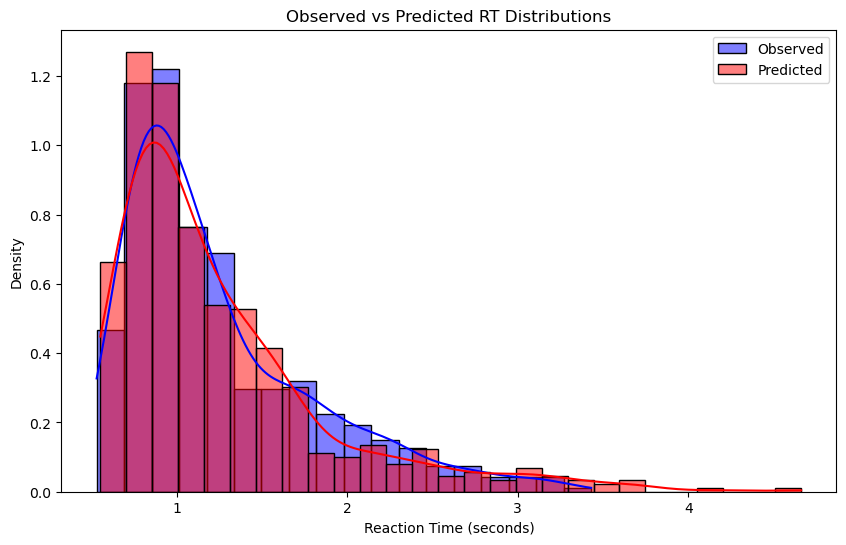
\includegraphics[scale=.4]{20_deg_obs_vs_pred.png}
    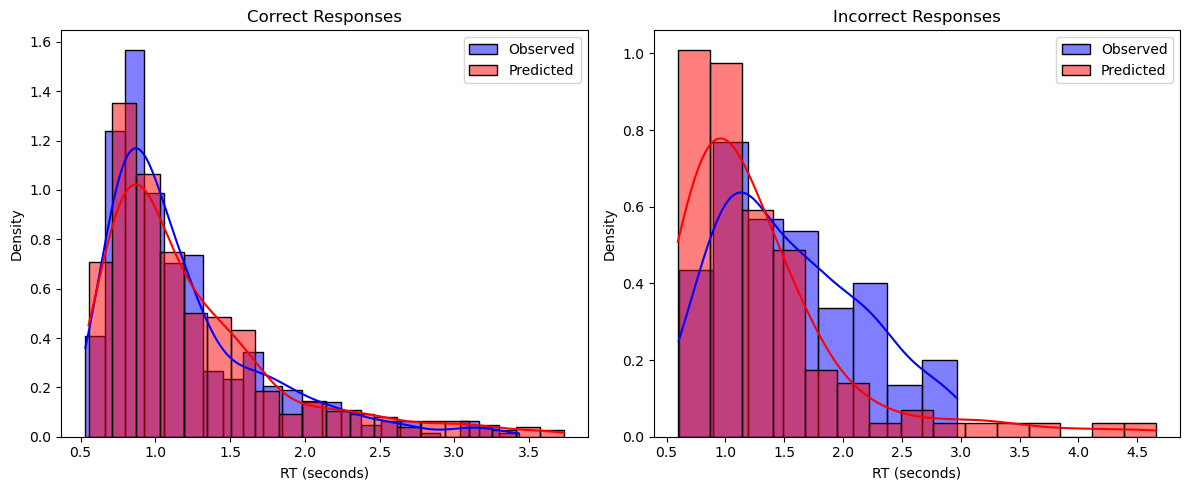
\includegraphics[scale=.4]{20_deg_obs_vs_pred_by_c.png}
    \caption{Graphs comparing the original and predicted RT distributions for the 20° condition.}
    \label{fig:20deg}
\end{figure}
\begin{figure}[ht]
    \centering
    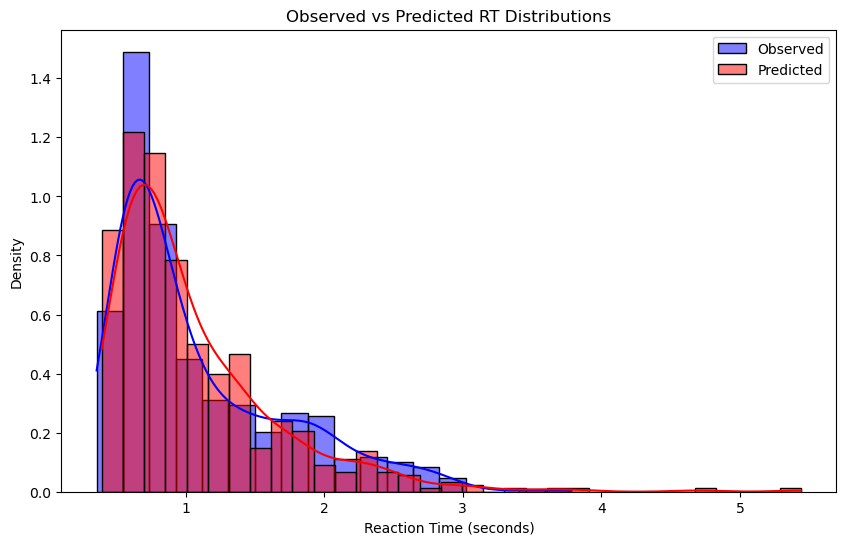
\includegraphics[scale=.4]{45_deg_obvs_vs_pred.png}
    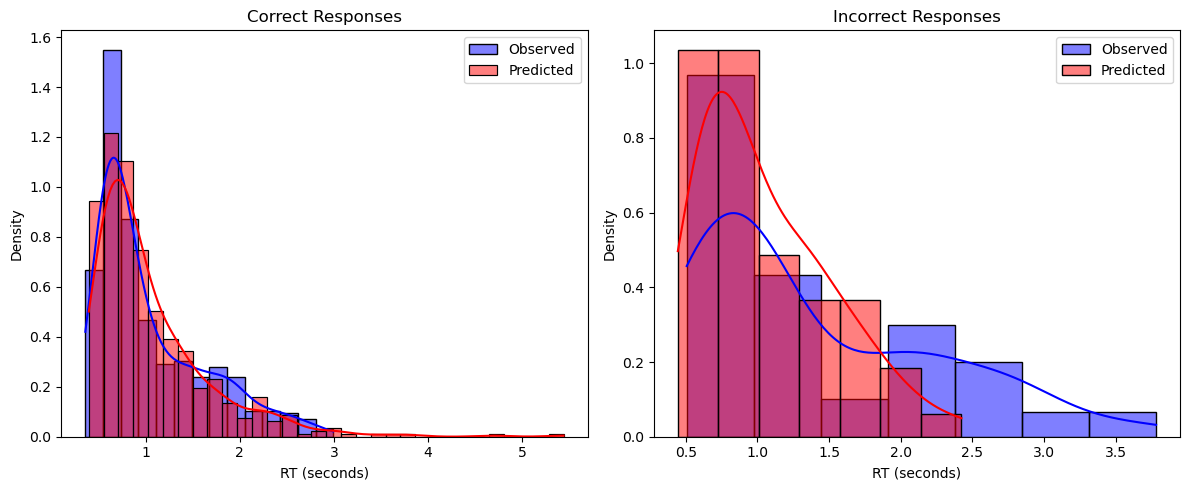
\includegraphics[scale=.4]{45_deg_obvs_vs_pred_by_c.png}
    \caption{Graphs comparing the original and predicted RT distributions for the 45° condition.}
    \label{fig:45deg}
\end{figure}

\section{Discussion}
Overall, our findings suggest that having a larger angle between axes makes the task easier for the participant. Despite the fact that the boundary separation is higher in the 45° version of the experiment, both the drift rate and non-decision time are lower, leading to slightly faster RTs overall. This result makes sense, seeing as a greater angle of separation would allow for easier discrimination of the motion of the balls at points close to where the axes intersect. The DDM parameters provide insights into the cognitive processes underlying decision-making in this task. The higher drift rate and lower non-decision time for the 45° condition suggest that participants accumulate evidence more rapidly and efficiently when the axes are more distinct. It is interesting to note that the boundary separation is higher in the 45° condition, which may indicate that participants are more cautious in their decision-making when the axes are more distinct. This could be due to a greater perceived risk of making an incorrect decision, leading to a more conservative approach. The starting bias remains similar across both conditions, suggesting that the participant's initial inclination toward one response option does not significantly change with the angle of the axes. This finding indicates that the participant's decision-making strategy is relatively stable, regardless of the task difficulty. That being said, these results are not exhaustive. Future studies have many potential improvements; for one, we could analyze the data from multiple participants to see if the results are consistent across individuals. Additionally, we could explore the effects of other variables, such as the previously mentioned focus on one or both axes, to see how they affect decision-making. Other models, such as a regression model, may be useful for determining which paramters has the greatest impact on accuracy and RT.

\bibliographystyle{plain}
\bibliography{refs}

\end{document}